% Author: Dun-Ming Brandon Huang
% bMail: dunmingbrandonhuang@berkeley.edu
% Question Source: Previous Exams
% Solution Source: Self

\qns{MINE COINS now they're steady-state now}

\textbf{Learning Topic}: Steady-State Transition System and Eigenanalysis \\
There is a population of cryptocurrency miners. These miners are primarily interested in two coins: OskiCoin and BearCoin, and they switch between mining the two coins in a predictable way. Every week, $20\%$ of OskiCoin miners switch to BearCoin and $30\%$ of BearCoin miners switch to OskiCoin. The remaining miners keep mining the same coin for the following week.\\
Let $s_{1}[n]$ be the number of miners of OskiCoin on week $n$ and $s_{2}[n]$ be the number of miners of BearCoin on week $n$:
\[\vec{s}_{1}[n] = \begin{bmatrix} s_{1}[n] \\ s_{2}[n] \end{bmatrix}\]

\begin{enumerate}
    \item\label{graph_drawing}{
        Draw a well-labeled directed graph showing how the population of miners changes each week. Be sure to label each node and place appropriate weights on each edge.
        
    }
    \meta{
        This question comes from Q9(a) of Spring 2018’s Midterm 1.
        
    }
    \ans{
        \begin{center}
            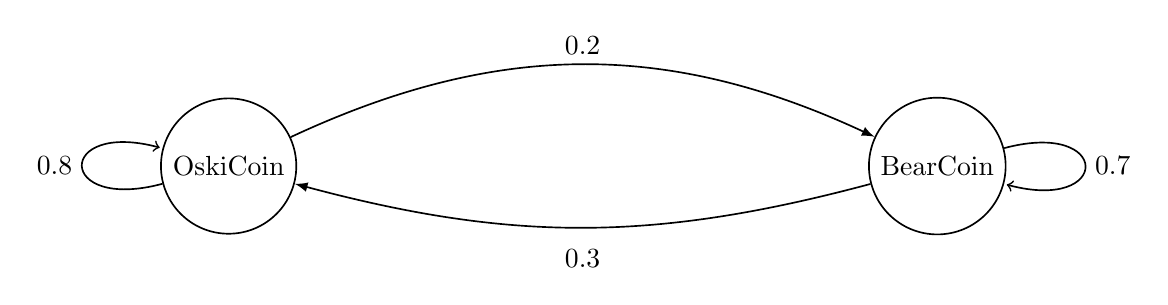
\begin{tikzpicture}[-latex, auto, node distance={9cm}, semithick, main/.style = {draw, circle}]
                \node[main] (A) {OskiCoin};
                \node[main] (B) [right of=A] {BearCoin};
                \path (A) edge [loop left] node[left] {$0.8$} (A);
                \path (A) edge [bend left =25] node[above] {$0.2$} (B);
                \path (B) edge [bend left =15] node[below=0.15cm] {$0.3$} (A);
                \path (B) edge [loop right] node[right] {$0.7$} (B);
            \end{tikzpicture}
        \end{center}

    }
    
    \item\label{matrix_identification}{
        Determine the state transition matrix $A$.
        
    }
    \meta{
        This question comes from Q9(b) of Spring 2018’s Midterm 1.
        
    }
    \ans{
        \[A=
        \begin{bmatrix}
            0.8 & 0.3 \\
            0.2 & 0.7
        \end{bmatrix}
        \]
        
    }
    
    \item\label{eigen_identification}{
        Find the eigenvalues and eigenvectors of $A$.
        
    }
    \meta{
        This question comes from Q9(c) of Spring 2018’s Midterm 1.\\
        
    }
    \ans{
        To find the eigenvalues of matrix $A$, we will solve the polynomial that is
        \begin{align*}
            \det{
                \begin{bmatrix}
                    0.8 - \lambda & 0.3 \\
                    0.2 & 0.7 - \lambda
                \end{bmatrix}
            } &= (\lambda - 0.8)(\lambda - 0.7) - (0.3)(0.2) \\
            &= \lambda^{2} - 1.5\lambda + 0.5 \\
            &= 0
        \end{align*}
        To solve that polynomial, we would attain the result $\lambda_{1}=0.5$, $\lambda_{2}=1$. We can either work with the quadratic formula or factor the above polynomial to reach here.\\
        Now we may attain the eigenvectors of each eigenvalue by making use of the property that
        \[(A-\lambda_{n}I)\vec{v_{\lambda_{n}}}=\vec{0}\]
        \textbf{Finding $\vec{v_{\lambda_{1}}}$:}\\
        \hspace*{\fill}\begin{minipage}{\textwidth-15mm}
            \[
            \begin{bmatrix}
                0.8 - 0.5 & 0.3 \\
                0.2 & 0.7 - 0.5
            \end{bmatrix} \vec{v_{\lambda_{1}}} = \vec{0}\]
            For a real value $n$, we can observe that
            \[\vec{v_{\lambda_{1}}} = \begin{bmatrix} n \\ -n \end{bmatrix} \]
            or, to be more straightforward, we can show one of its possible eigenvectors, which we will do with the next case as well for brevity:
            \[\vec{v_{\lambda_{1}}} = \begin{bmatrix} 1 \\ -1 \end{bmatrix} \]
        \end{minipage}
        
        
        \textbf{Finding $\vec{v_{\lambda_{2}}}$:}\\
        \hspace*{\fill}\begin{minipage}{\textwidth-15mm}
            \[
            \begin{bmatrix}
                0.8 - 1 & 0.3 \\
                0.2 & 0.7 - 1
            \end{bmatrix} \vec{v_{\lambda_{2}}} = \vec{0}\]
            We can observe that one of the possible eigenvectors is:
            \[\vec{v_{\lambda_{2}}} = \begin{bmatrix} 3 \\ 2 \end{bmatrix} \]
        \end{minipage}
        
    }
    
    \item\label{linear_combination}{
        Express $\begin{bmatrix} 5 \\ 0 \end{bmatrix}$ as a linear combination of the eigenvectors, $\mathbb{V} = \{v_{1}, \dots, v_{n}\}$.
        
    }
    \meta{
        This question comes from Q9(d) of Spring 2018’s Midterm 1.
        
    }
    \ans{
        We look for coefficients $\alpha_{1}$ and $\alpha_{2}$ such that
        \[\begin{bmatrix} 5 \\ 0 \end{bmatrix} = \alpha_{1}\vec{v_{\lambda_{1}}} + \alpha_{2}\vec{v_{\lambda_{2}}}\]
        or, as well as expressed to be
        \[
        \begin{bmatrix}
            \vec{v_{\lambda_{1}}} & \vec{v_{\lambda_{2}}}
        \end{bmatrix}
        \begin{bmatrix} \alpha_{1} \\ \alpha_{2} \end{bmatrix} =
        \begin{bmatrix} 5 \\ 0 \end{bmatrix}
        \]
        Solving the system, we get that $\alpha_{1}=2$ and $\alpha_{2}=1$.\\
        Therefore:
        \[\begin{bmatrix} 5 \\ 0 \end{bmatrix} = 2\vec{v_{\lambda_{1}}} + \vec{v_{\lambda_{2}}}\]
        
    }
    
    \item\label{steady_state_distribution}{
        If we start with $1000$ miners mining OskiCoin and $0$ miners mining BearCoin, then what will the steady state distribution of miners be?
        
    }
    \meta{
        This question comes from Q9(e) of Spring 2018’s Midterm 1.\\
        This sequence of questions are standard templates of any steady state eigen-analysis problems that have also been brought up in the homework assignments and discussion sections.
        
    }
    \ans{
        Let us first attempt to find and express the initial state as a linear combination of state transition matrix's eigenvectors.\\
        The initial state, according to how the problem is defined, would be the vector that contains the number of OskiCoin miners, then the number of BearCoin miners, providing
        \[\vec{s}[0] = \begin{bmatrix} 1000 \\ 0 \end{bmatrix}\]
        We see that $\vec{s}[0]=200\begin{bmatrix} 5 \\ 0 \end{bmatrix}$, therefore, we have discovered that
        \[\vec{s}[0] = 400\vec{v_{\lambda_{1}}} + 200\vec{v_{\lambda_{2}}}\]
        The steady state distribution can be stated as the vector resulting from having the initial state $\vec{s}[0]$ undergoing nearly infinite times of transformation (based on the transition matrix $A$, and by transformation we mean multiplying by $A$!). The above statement can be mathematically expressed as
        \[\lim_{t\to\infty}\vec{s}[t] = \lim_{t \to \infty}A^{t}\vec{s}[0]\]
        Let us now attempt to evaluate the steady state distribution:
        \begin{align*}
            \lim_{t\to\infty}\vec{s}[t]
            &= \lim_{t\to\infty}A^{t}\vec{s}[0] \\
            &= \lim_{t\to\infty}A^{t}(400\vec{v_{\lambda_{1}}} + 200\vec{v_{\lambda_{2}}}) \\
            &= \lim_{t\to\infty}(400\lambda_{1}^{t}\vec{v_{\lambda_{1}}} + 200\lambda_{2}^{t}\vec{v_{\lambda_{2}}}) \\
            &= 200\vec{v_{\lambda_{2}}} = \begin{bmatrix} 600 \\ 400 \end{bmatrix}
        \end{align*}
        Therefore, the steady state distribution is 
        \[\lim_{t\to\infty}\vec{s}[t] = \begin{bmatrix} 600 \\ 400 \end{bmatrix}\]
    }

\end{enumerate}